\documentclass[conference]{IEEEtran}
\IEEEoverridecommandlockouts

\usepackage{cite}
\usepackage{amsmath,amssymb,amsfonts}
\usepackage{algorithmic}
\usepackage{graphicx}
\usepackage{textcomp}
\usepackage{xcolor}



\def\BibTeX{{\rm B\kern-.05em{\sc i\kern-.025em b}\kern-.08em
    T\kern-.1667em\lower.7ex\hbox{E}\kern-.125emX}}
\begin{document}

\title{Scrum vs Kanban: Comparative analysis for most suited approach for Software Development\\
}

\author{\IEEEauthorblockN{ Kajal Lochab}
\IEEEauthorblockA{\textit{Institute of Technology} \\
\textit{Nirma University}\\
Ahemdabad , India \\
21bce103@nirmauni.ac.in}
\and
\IEEEauthorblockN{ Kapil Mehta}
\IEEEauthorblockA{\textit{Institute of Technology} \\
\textit{Nirma University}\\
Ahemdabad , India\\
21bce148@nirmauni.ac.in}
\and
\IEEEauthorblockN{ Harsh Parekh}
\IEEEauthorblockA{\textit{Institute of Technology} \\
\textit{Nirma University}\\
Ahemdabad ,India \\
22bce524@nirmauni.ac.in}
}

\maketitle

\begin{abstract}
In the vast realm of software development, we've progressed through different eras of project management, transitioning from rigid methodologies like Waterfall and Vee models to embracing agile practices. These Agile methodologies, born out of the need for adaptability in an ever-changing landscape, have emerged as transformative forces in software project management. Among the champions of this Agile revolution, we find Scrum and Kanban, two stalwart methodologies renowned for their prowess in managing software projects. Scrum and Kanban, both offspring of the Agile movement, have solidified their positions as primary project management approaches in the software development domain. They provide strategic frameworks for task identification, team coordination, and efficient time management, crucial elements in project execution. However, as we embarked on our exploration of the extensive literature, we encountered a significant challenge, akin to a mystery. This challenge revolves around the scarcity of comprehensive statistical data, leaving a lingering question regarding which approach holds a definitive edge over the other. The question of which method excels in areas like budget management, quality assurance, risk mitigation, scope definition, and schedule adherence remains without a clear answer. Yet, our expedition wasn't in vain. It revealed a treasure trove of qualitative insights. Both Scrum and Kanban have demonstrated their potential to nurture and deliver successful projects. The choice between these Agile giants is not a stark binary decision; it's an opportunity for a nuanced understanding. It's an invitation to embrace adaptability, foster effective teamwork, and make informed decisions. In the ever-changing landscape of software development, where adaptability reigns supreme, the Scrum vs. Kanban debate isn't a mere academic exercise. It's a journey, an exploration of the intricacies and strengths inherent in these methodologies. Our paper serves as your guide, leading you through this domain, and encouraging you to embark on your quest for project management excellence, with Scrum and Kanban as your trusted companions.
\end{abstract}


\begin{IEEEkeywords}
Software Engineering, Agile Software Development, Scrum, Kanban, SLR, Scrumban
\end{IEEEkeywords}

\section{Introduction}
% This document is a model and instructions for \LaTeX.
% Please observe the conference page limits.
In the ever-evolving world of software development, we can trace our journey through the annals of history—from the construction of China's monumental Great Wall, the grandeur of Egypt's Pyramids, to the audacious Apollo Space Program that marked the 1980s \cite{kwak2005brief}. With each era, the demands and intricacies of project development have shifted, ultimately culminating in our contemporary digital age \cite{seymour2014history}. Throughout this dynamic evolution, one constant remains steadfast: change \cite{kabeyi2019evolution}.

The relentless march of time brings with it shifting market needs, technological evolution, and the ever-changing landscapes of project environments \cite{padalkar2016six}. In this turbulent domain of software creation, agility becomes not just a preference \cite{dybaa2008empirical} but a necessity \cite{abrahamsson2017agile}. The need to adapt swiftly, navigate complex domains, and meet market demands with shorter development cycles and cost-effective solutions has given birth to many agile approaches and methods \cite{misra2012agile, rigby2016secret}.

Among the pantheon of agile methodologies \cite{rasnacis2017method, coram2005impact}, two luminaries stand out in the software development arena —Scrum\cite{schwaber2001agile} and Kanban \cite{ahmad2013kanban}. Born out of the need for agility in the face of the limitations of traditional methodologies like the Waterfall model \cite{thesing2021agile, amlani2012advantages} along with other incremental \cite{hibbs2009art} and iterative models \cite{mitchell2009comparison}, these agile titans have revolutionized the way software projects progress \cite{al2020agile}. 

Scrum, an agile framework that emerged as a response to the shortcomings of Waterfall, introduces a structured approach to development with its iterative and incremental cycles. In disparity, Kanban pulls motivation from the Lean Manufacturing and Toyota Production System, emphasizing visualizing workflow and maintaining a steady, efficient pace of work.

The choice of a development approach wields substantial influence over the outcome of software projects \cite{despa2014comparative}. It's a decision that has sparked a long-standing debate regarding the preference for either Scrum or Kanban \cite{lei2017statistical}. Such deliberations necessitate a profound understanding of these methodologies, including their strengths and weaknesses, limitations, relative advantages in different contexts, and more \cite{zayat2020framework}.

Both Scrum and Kanban come with their unique sets of challenges. Scrum may grapple with issues such as limited work visibility, local optimization, scalability hurdles, and shifting task priorities. Similarly, Kanban faces its problems and challenges \cite{ahmad2016transition}.

\begin{figure*}[]
    \centering
    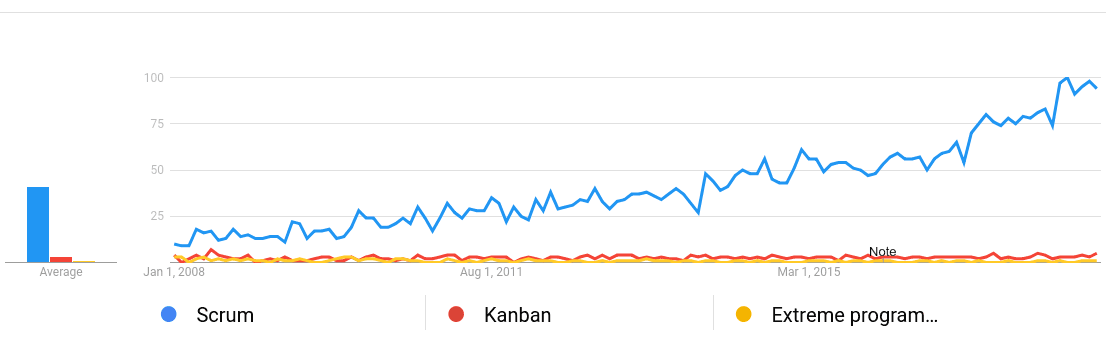
\includegraphics[width=0.8\linewidth]{trends.png}
    \caption{Scrum vs Kanban throughout the years}
    \label{fig: Trend for Scrum vs Kanban}
\end{figure*}

In the quest for optimization, some have proposed an intriguing idea: blending Scrum and Kanban, utilizing the strengths of both to mitigate their limitations \cite{ladas2009scrumban}. This fusion of agile methodologies has gained traction as a promising approach, offering the potential to complement each other's strengths \cite{reddy2015scrumban}.

While several literature reviews have explored the realms of Scrum \cite{cho2010exploratory, faniran2017adopting} and Kanban \cite{kirovska2015usage, ahmad2013kanban, ahmad2018kanban} individually, the need for a comprehensive comparison and integration of these methodologies to guide further research and practice remains largely unaddressed. It is within this uncharted territory that we embark on our journey—a journey to unravel the intricacies of Scrum and Kanban, explore their potential synergies, and light the way for future exploration and innovation in agile software development.

\subsection{Research Objectives}
\begin{enumerate}
  \item \textbf{Comparative Analysis:} To conduct an in-depth relative study of the Scrum and Kanban methods in software development. This analysis will involve understanding the core principles, strengths, weaknesses, and the situations where each methodology excels.

  \item \textbf{Integration Possibilities:} To explore the potential for integrating Scrum and Kanban, leveraging their respective strengths to mitigate limitations. This will involve identifying scenarios where a combined approach might yield better results than using each methodology independently.

  \item \textbf{Identifying Best Practices:} To identify best practices and guidelines for utilizing Scrum and Kanban in software development. This involves understanding how these methodologies can be tailored to suit different project contexts and deliver optimal results.

  \item \textbf{Framework for Decision-Making:} To develop a decision-making framework for choosing between Scrum and Kanban based on the project's specific requirements, limitations, and constraints.

  \item \textbf{Future Directions:} To give ideas on where more research, new ideas, and useful applications can be accomplished in the domain, taking into account how technology and market needs are always changing.
\end{enumerate}

\subsection{Research Contributions}
This research aims to construct the subsequent grants to agile software development:

\begin{enumerate}
  \item \textbf{Comprehensive Comparison:} By conducting an extensive comparative analysis of Scrum and Kanban, this research will offer a holistic view of these methodologies, helping practitioners and researchers make informed decisions.

  \item \textbf{Integration Insights:} By exploring integration possibilities, we will provide insights into how combining Scrum and Kanban can address the limitations of each methodology, opening avenues for improved project management.

  \item \textbf{Best Practice Guidelines:} This research will offer practical guidelines and best practices for effectively implementing Scrum and Kanban in software development, enhancing the applicability and adaptability of these methodologies.

  \item \textbf{Decision-Making Framework:} The development of a decision-making framework will empower project managers and teams to select the most suitable methodology based on their project's unique requirements and constraints.

  \item \textbf{Future Research and Innovation:} By shedding light on potential future research directions and emerging trends in the domain, this study strives to scintillate innovation and inspire further exploration of this dynamic field.
\end{enumerate}

Through these research objectives and contributions, we aspire to provide valuable insights and practical knowledge that will benefit the software development community and foster advancements in agile methodologies.

\subsection{ORGANIZATION OF THE PAPER}

This is how the paper is organized. Section I explores the history of project management and states how Scrum and Kanban came into the stage of software development. It also explains existing research work done in this direction and lists its research contributions. Section II summarizes the methodology of the research. Section III states the literature review of the research about how other existing research has contributed to the Scrum vs Kanban. Section IV draws out the comparative analysis of both approaches. Section V shows Empirical Studies and Case Examples carried out in the direction of the research. Section VI gives the conclusion of the work in brief.

\section{Methodology}

\subsection{Why SCRUM or KANBAN?}

The preference between Scrum and Kanban in software engineering (SE) relies on diverse facets, including the team's precedences, the project's traits, and the objectives of the development cycle. This judgment can significantly influence how a team manages its work, cooperates, and furnishes value. In this section, we will examine the grounds for specifically choosing Scrum or Kanban in SE.\cite{kniberg2010kanban}

Scrum is a well-established Agile framework with distinguishable roles, accountabilities, and a structured strategy for project management. It is specifically applicable when:\cite{kniberg2010kanban}

\begin{itemize}
\item \textbf{Prefer Prescribed Methods:} When Agile team associates favour a structured and authoritarian approach, Scrum is an appropriate preference. Scrum depicts roles like Scrum Master, Development Team and Product Owner individually with separate duties\cite{s1-alqudah2018empirical}\cite{kniberg2010kanban}.

\item \textbf{Team Size and Batching:} Scrum functions well for teams incorporating 5-11 development associates, and it concentrates on managing work into one-, two, or four-week sprints. If your project fits specific standards, Scrum is a feasible choice\cite{s1-alqudah2018empirical}\cite{mahnivc2015scrum}.

\item \textbf{Estimation and Prioritization:} Scrum emphasizes estimating work and prioritization based on the sprint's length. If your project requires this approach to managing requirements and tasks, Scrum is a suitable choice\cite{s1-alqudah2018empirical}.

\item \textbf{Emphasis on Knowledge and Decision Making:} Scrum fosters knowledge sharing, understanding, and judgment-making established on what is comprehended. If your project meets these aspects above cost-saving and lead-time deduction, Scrum is more suitable\cite{s1-alqudah2018empirical}\cite{mahnivc2015scrum}.
\end{itemize}

Kanban, on the other hand, is a more adjustable and less rigid method that accentuates envisioning the creation procedure and optimizing flow. It is well-suited for the following scenarios:

\begin{itemize}
\item \textbf{Preference for Flexibility:} When Agile team associates favour a more adaptable approach with fewer predefined functions and accountabilities, Kanban is a satisfactory fit. Kanban does not have specified roles like Scrum \cite{s1-alqudah2018empirical}\cite{kniberg2010kanban}.

\item \textbf{Small Team Size and Continuous Flow:} Kanban can be embraced by smaller groups of 3-14 members, and it allows for work to be batched on a daily or even hourly basis. If your team requires ongoing prioritization and flexibility, Kanban is a fitting option\cite{s1-alqudah2018empirical}\cite{kniberg2010kanban}.

\item \textbf{Focus on Cutting Lead Time and Cost Saving:} Kanban places a strong priority on decreasing lead times and cutting costs, particularly for functions. If these ideals align with your project objectives, Kanban is a more suitable alternative\cite{s1-alqudah2018empirical}.

\item \textbf{Emphasis on Quality:}  Kanban emphasizes enhancing quality producing a good choice when quality is a top priority\cite{s1-alqudah2018empirical}.
\end{itemize}

In summary, the choice between Scrum and Kanban in software engineering depends on diverse aspects, including team choices, project size, need for flexibility, focus on cost redemptions, and assertiveness on quality. While Scrum provides configuration and well-defined roles, Kanban delivers more flexibility and steady flow. Additionally, Scrumban, a hybrid approach combining Scrum and Kanban, can be assessed for Agile teams that want to combine both to adapt to changing situations. The conclusion should be established by carefully assessing the project's distinctive prerequisites and constraints.\cite{abrahamsson2017agile}

\subsection{What is Scrum?}
\begin{figure}[h!]
    \centering
    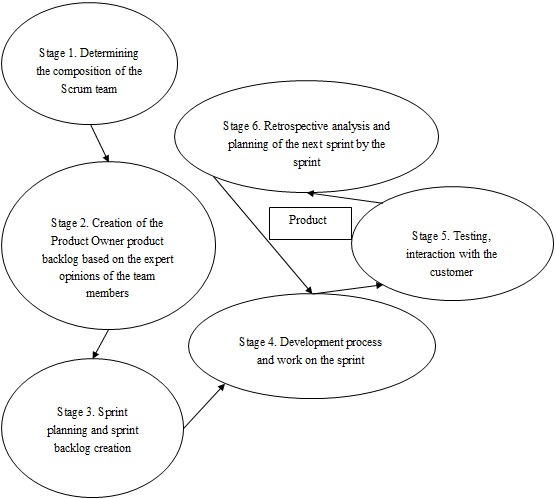
\includegraphics[width=1\linewidth]{s1.jpg}
    \caption{Scrum Overview}
    \label{fig:Scrum}
\end{figure}



Scrum stemmed from industrial procedure control ideas and has been widely embraced in the software endeavour. It is an Agile software development approach indicated by its emphasis on collaboration, adaptability, and iterative development. Scrum fosters a team-based strategy for project management, where diminutive, cross-functional teams work closely to attain a shared goal. Here is a straightforward overview of Scrum\cite{schwaber1997scrum}:


Roles in Scrum:
Scrum defines specific roles within the development process:

\begin{itemize}
\item \textbf{Scrum Master:} It is accountable for guaranteeing that the unit clings to the practices of Scrum. They manage Scrum events, submit changes to improve the team's productivity and function as a compass for the unit\cite{schwaber1997scrum}.

\item \textbf{Product Owner:} It is the tryst connecting the product crew and project stakeholders. Their duties include gathering and prioritizing prerequisites, managing the Product Backlog, and guaranteeing that the derivative aligns with stakeholder requirements\cite{rising2000scrum}.

\item \textbf{Development Team:} The team incorporates three to nine self-organizing, cross-functional developers. They are accountable for enforcing the product's prerequisites and furnishing a functional software product incrementally\cite{rising2000scrum}.
\end{itemize}


Sprints:
Scrum works in Sprints, which are iterative cycles usually lasting two to four weeks. The subsequent events denote sprints\cite{diebold2015practitioners}:

\begin{itemize}
\item \textbf{Sprint Planning:} The Product Owner, at the start of Sprint, demonstrates the most elevated primacy backlog items. The Development Team evaluates how many can be completed in the forthcoming Sprint, and this impacts creating a Sprint Backlog, which contains the essentials the team is devoted to achieving during the Sprint\cite{diebold2015practitioners}\cite{rigby2016secret}.

\item \textbf{Daily Scrum:} In a proceeding Sprint, the Development unit drives a day-to-day Scrum meeting, typically fifteen minutes and guided by the Scrum Master. In the meeting, team members respond to three key questions: What did they achieve yesterday to function toward the Sprint goal? What will they do today to drive closer to the Sprint goal? Have they experienced any issues that might hamper advancement\cite{diebold2015practitioners}?

\item \textbf{Sprint Review:}The team executes a Sprint Review at the end of Sprint to present Sprint's by-products to stakeholders. These results are estimated against a typical definition of "Done." Stakeholders furnish feedback, and additional progress is examined\cite{diebold2015practitioners}\cite{schwaber1997scrum}.

\item \textbf{Sprint Retrospective:} The Development Team holds a Sprint Retrospective to deliberate on Sprint's performance, pinpoint concerns, and devise solutions for persistent improvement\cite{schwaber1997scrum}
\end{itemize}.


Scrum's focus on little, self-organizing teams, time-boxed development, and periodic stakeholder exchanges allows for constructing an observable, functional product increment after each Sprint. This incremental technique allows on-time delivery, continuous customer feedback, and the development of a coordinated and trust-building culture within the team. Scrum delivers a structured but adaptive framework for software development, accentuating the delivery of value and consumer delight\cite{diebold2015practitioners}.


\subsection{What is Kanban?}
\begin{figure}[h!]
    \centering
    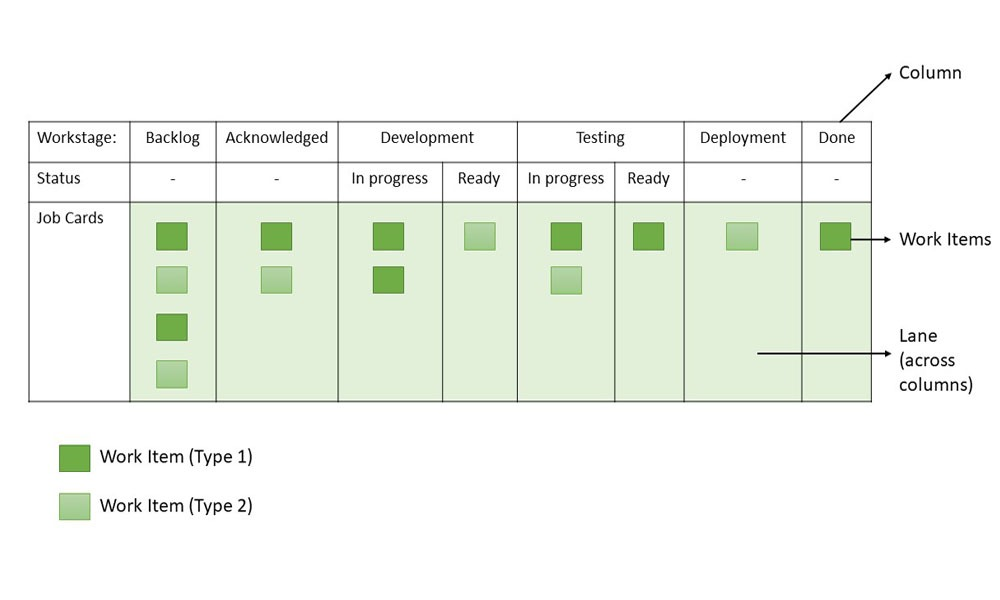
\includegraphics[width=1\linewidth]{k1.jpg}
    \caption{Kanban Overview}
    \label{fig:Kanban}
\end{figure}
Kanban is a software development method that has acquired growing engagement, particularly in lean product growth. Like Scrum, Kanban proposes a framework for teams to govern and optimize their work methodologies. However, Kanban sets a powerful stress on minimizing scrap, improving workflow visualization, and furnishing flexibility to adjust to evolving needs.\cite{corona2013review}

Kanban is created on many core principles and practices, each donating to its significance:

\begin{itemize}
\item \textbf{Visualization:} One of the foremost doctrines of Kanban is envisioning the work process. This is often accomplished via a Kanban board, which depicts the different phases of work as queues and individual assignments or work articles as cards. Team members can glimpse what is in progress, what is remaining, and what has been achieved\cite{ikonen2010leadership}\cite{ikonen2011impact}.

\item \textbf{Limiting Work in Progress (WIP):} Kanban restrains the amount of tasks in advance for any moment in time. It averts overburdening team members and maintains a continued workflow. It also emphasizes bottlenecks and zones that need engagement\cite{ikonen2010leadership}.

\item \textbf{Pull system:} Kanban works as a pull system, where assignment is pulled through the system founded on customer demand. This deviates from classic push systems, guaranteeing that work is yielded fast and not prematurely\cite{ikonen2011impact}.

\item \textbf{Continuous Improvement:} Kanban facilitates teams to enhance their processes frequently. Periodic feedback and retrospective meetings assist in determining problems, acclimating to changing requirements, and improving efficiency\cite{ikonen2011impact}.

\item \textbf{Customer Focus:} The Kanban technique holds the customer at the fore. Work items are pulled based on customer demand, and feedback is gathered regularly to align evolution with customer needs\cite{al2015kanban}.

\item \textbf{Self-Organization:} Kanban encourages self-organizing teams, permitting members to select and organize their work tasks. This grant fosters more significant accountability and ownership\cite{corona2013review}
\end{itemize}.


Kanban's workflow process consists of the following stages:

\begin{itemize}
\item \textbf{Visualization:} The Kanban board is set up, showing queues illustrating stages of work, such as "To-Do," "In Progress," and "Done." Work items are illustrated as cards on the board\cite{ikonen2010leadership}.

\item \textbf{WIP Limits:} Each step on the Kanban board has a predefined boundary for the amount of work entities in that set simultaneously\cite{al2015kanban}.

\item \textbf{Pulling work:} Team members pull work items from the "To-Do" queue into the "In Progress" queue to guarantee they do not transcend the WIP limit\cite{al2015kanban}.

\item \textbf{Continuous Improvement:} Teams regularly meet to examine advancement, recognize issues, and make refinements. Feedback is gathered from customers and stakeholders\cite{ikonen2011impact}.
\end{itemize}

In conclusion, Kanban offers a pliant and adaptive approach to software development, highlighting waste reduction, workflow visualization, and customer-centric techniques. This approach is endearing when negotiating with developing prerequisites and complex projects\cite{corona2013review}.


\section{Literature Review}
In this comprehensive review, we synthesize the key insights from three research papers of Scrum Methodology, three research of KANBAN Methodology and six research papers on Comparative study on Scrum Vs Kanban.

\subsection{Scrum}
1. The paper \cite{scrump1} states the agile methodologies  in software development using the Scrum model. It emphasizes the benefits of adopting agile development over more conventional approaches, such as waterfall or prototype, and how Scrum is a simple way to put agile into practice. In order to strengthen the Scrum process, the document also highlights the advantages of improved work traceability, good team communication, and the significance of retrospection following each sprint. Additionally, the document suggests a new Scrum model that may assist in removing the Scrum model's existing drawbacks. The suggested approach calls for the formation of a Scrum team, team training, sprint planning, timed delivery, daily scrum, and retrospection. Time-boxed and creative activities are also included in the suggested model to increase the Scrum process's effectiveness.
This paper states the advantages of agile development, namely the Scrum paradigm, for the development of customized software. It stresses the model's adaptability, early delivery, and flexible life cycle.It thinks Scrum may help firms develop and meet CMM standards, even while acknowledging that there are substantial backlogs and areas for improvement in its implementation—such as a lack of automation, stronger management support, and experienced team members.
\newline
\newline
\begin{enumerate}
\item\textbf{Introduction}: An introduction to the significance of the creation of software in information technology businesses.The difficulty of creating new software and the requirement for expansion in multiple dimensions
The advantages of using an agile methodology for the development of individualized products
The widespread use of the agile development framework known as Scrum.
\item\textbf{Method of Study}:
The requirement for an improved Scrum model that is capable of operating on its own.
The advantages that come along with Scrum's adaptable flexibility and early delivery
The idea is that businesses can achieve maturity through agile adaption and that this helps them achieve higher CMM levels
The many frameworks for agile development, with Scrum being the one that's easiest to put into practice.
There is a possibility that Scrum will become the most in-demand approach for development without causing any headaches.
\item \textbf{A Review of Current Literature}:
A synopsis of Scrum's inception and evolution
Scrum is considered in relation to other agile development models, such XP and Kanban.
One of the benefits and drawbacks of implementing Scrum is the need for qualified and experienced team members and Scrum masters.
 \item \textbf{Conclusion}: 
The capacity of Scrum to respond to the requirements of thousands of projects and to be expanded to accommodate vast amounts
The less significant facets of the Scrum implementation that require refinement, such as the absence of automation in workflow and testing, the need for more management support, and the availability of skilled team workers.
The new model for Scrum, which has been presented, will make Scrum a more all-encompassing strategy than existing agile approaches, with distinct approaches to handling traditional and innovative jobs.
The flexibility of Scrum to be applied to any industry and produce solutions that are both successful and sustainable.
 \newline
 \newline
2.In the paper\cite{scrump2}, the Scrum technique with agile methodologies, which has been studied since the 1990s and is still a mainstay in many fields, is examined via a systematic literature review. The research provides a concise comparison of traditional project management approaches with agile project management methodologies, highlighting and explaining the primary distinctions between the two. The agile approaches incorporate both quantitative and qualitative data, displaying elements of the Scrum framework. The study's background is given, a brief theoretical framework is given, details of the research method used are given, the SLR method is used, the results are analyzed, and the paper ends with citations of relevant literature.
\newline
\newline
The SLR technique is a method that is commonly used in exploratory research that creates guidelines. This is due to the fact that the SLR approach covers searching, selecting, critically assessing, and making synopses of the outcomes of primary research. Two groups of researchers, \cite{scrump2} and \cite{al2020agile}, made structures that hold the main steps of literature analysis. They did this to make SLR a standard method and to stop research and data analysis from being skewed. The author of the article [27] carried out a paper in order to compile the important success criteria of both the motivator and the demotivator of agile software development.
\newline
\newline
Steps of the SLR, as outlined in \cite{scrump2}, are discussed throughout the article, beginning with the planning of the review. According to the paper, the initial stage of the SLR is concerned with the planning of reviews. The researchers highlight two first elements that are essential for preparing for the review stage, which are as follows: a) specifying the research topic; and b) developing a study methodology. Both of these are mentioned as being crucial. The author's statements found in \cite{scrump1} served as a foundation for the development of the research questions. The researchers raise some thought-provoking concerns that can be investigated further with SLR.

The research highlights the importance of project management by highlighting the fact that it was developed as a response to issues that occurred from poorly executed projects. Additionally, the knowledge provided by this research might be helpful to those in the domains of industrial engineering and computer science. We came to the conclusion that Scrum is an adaptable framework for the creation of projects with an empirical foundation based on the results. Its creator, Jeff Sutherland, first introduced the methodology in the 1990s. It is a methodology that is both flexible and adaptable.
\newline
\newline
In this paper, a literature review is conducted on the topic of contrasting traditional approaches with agile ones, with a specific emphasis placed on the Scrum framework. The study draws attention to the increasing significance of using agile approaches in project management, particularly in the domains of industrial engineering and computer science. Numerous studies have been conducted to investigate the ideas, methods, and results associated with the Scrum framework, which has become one of the most renowned and extensively used approaches within the agile landscape. The findings are put into context by the study in a way that is directly relevant to the requirements and concerns of professionals working in these disciplines. The research comes to the conclusion that Scrum is a potentially useful approach for the creation of empirically-based projects because to the inherent flexibility and adaptability of the framework. This methodology and its consequences for project practitioners and researchers will be dissected in great detail throughout the course of this paper.
\newline
\newline
This article provides an overview of Scrum, an agile methodology for developing empirically-based projects that is most commonly utilized in the field of computer science. This article places an emphasis on the relevance of project management and contains information that is pertinent to professionals in the fields of industrial engineering and computer science. On the other hand, one of the disadvantages of the study is that it is based on a systematic literature evaluation of only 41 papers, which might not cover the whole spectrum of the issue. In addition, it does not offer a full overview of the subject matter but rather focuses on particular areas of Scrum. In future studies, it is important to look into how Scrum can be used in different situations, what problems it might cause, and how it stacks up against other agile project management methods. The paper discusses Scrum, an agile framework for empirical-based project development primarily used in computer science. It emphasizes the importance of project management and provides relevant information for professionals in industrial engineering and computer science. However, the study's limitations include a systematic literature review of 41 articles, which may not represent the entire scope of the topic. It also does not provide a comprehensive overview of the topic, focusing on specific aspects of Scrum. Future studies should explore Scrum's applicability in various areas, address identified problems, and compare it with other agile methodologies for project management.
\newline
\end{enumerate}

3. The paper \cite{scrump3} provides a review of the key studies that report employing Scrum methods in Global Software Development projects. This review is presented in the form of a systematic literature review. The purpose of this study is to identify the obstacles that are associated with utilizing Scrum for Global software Development  projects and the potential techniques for overcoming those challenges.

After using a search strategy, the researchers found 366 documents, 20 of which were found to be primary papers that were relevant to their investigation. They used the material from the publications to learn about the many issues that arise while applying Scrum in GSD as well as the current fixes for these issues. The review's conclusions are summed up in this paper, which should aid academics and industry professionals in comprehending the difficulties involved in applying Scrum to GSD projects and the solutions available to address those difficulties.


The analysis concentrates on the increasing attraction to involving agile methods in GSD initiatives and the writings on employing Scrum. It is a considerably distinguished agile technique in dispersed growth projects. The paper also highlights the increasing inquisitiveness in involving agile methods in GSD undertakings. The researchers came to the conclusion that even though there are many challenges involved, there have been some successful implementations of agile practices with distributed teams. Other scholars, on the other hand, maintain that the fundamental question of whether or not agile approaches can be employed in a distributed system is still up for debate.

The report notes a number of difficulties associated with the use of Scrum in GSD, including communication difficulties, cultural differences, changes between time zones, and the absence of face-to-face engagement. The researchers also mention contemporary solutions to cope with these issues, such as the establishment of various communication lines, the modification of Scrum processes, the utilization of stringent communication regulations, and the requirement of involvement.

The study's conclusion notes that using agile approaches in projects related to GSD is becoming more and more popular. Additionally, a growing corpus of research papers has examined the many organizations, issues, and application scenarios for agile approaches in GSD projects. To far, there hasn't been much effort put into methodically identifying, creating, and delivering the findings that have been established on the advantages of Scrum methods in GSD.

\begin{enumerate}
    \item \textbf{Introduction}: is obscured in this area of the paper, the writer presents the reader with the increasing pull to embrace agile principles for GSD projects. This section is responsible for setting the stage for the reader. It draws attention to the fact that there is currently a research void addressing the precise agile methods that are beneficial for GSD. It is explained that the primary purpose of this study is to carefully look over all the preliminary examinations that converse concerning using Scrum principles in Grand Design projects. It is important to stress the significance of this research so that the upcoming portions can be comprehended without any confusion.
\newline
\item \textbf{Background and Motivation}: This portion will serve as the basis for the rest of the research. It outlines the Scrum methodology and explains its primary tenets as well as the practices that are associated with it. The background of dispersed teams and projects is set, and the complexities and issues that come along with them are illustrated using Global Software Development as an example. An explanation of why a literature study is needed is given, with a focus on the need to gather and look into previous research and experiences related to Scrum in GSD. It also sheds information on the more widespread movement toward an interest in agile approaches in GSD, so laying the groundwork for the subsequent concentration on Scrum.
\newline
\item \textbf{Research Methods}: This publication presents a systematic literature analysis of primary studies on Scrum processes for GSD projects. The review aims to locate, compile, and discuss the findings on the use of Scrum methods for GSD. The search method used was a predetermined search technique, exploring  e-databases like the ACM Digital Library, IEEE Xplore, and Scopus. The search narrowed to publications published between 2000 and 2009, with English as the language of choice. The review identified 366 publications, with 20 being primary papers relevant to the investigation. The researchers used a pre-defined data extraction form to collect information from the chosen studies. Due to the lack of a structured structure, conflicts were resolved through consensus-building meetings and consultation with a third independent researcher. The primary studies were classified based on distributed project contextual elements and project frequencies. The majority of studies reported Scrum implementation in intra-organizational, global organizations, with a limited number of distributed sites involved.

\item \textbf{Results}: The effects of the extensive literature study are delivered in this area of the paper. It discusses the difficulties that crop up as a result of employing Scrum in GSD projects as well as the solutions that have been gleaned from previous research to deal with these difficulties. In this section, a summary of the key studies that have reported the implementation of Scrum principles in GSD is provided with the purpose of providing readers with insights into the existing body of knowledge in this field.

\item \textbf{Discussions}: In this section of the report, the findings from the literature review are analyzed and discussed in depth. It provides an in-depth analysis rather than only providing the results, which is a significant step up from the former. In this work, we investigate the implications of the findings for the efficiency with which Scrum may be used in GSD projects. It is possible that it will explore ways in which the difficulties that were found might be reduced, as well as lessons that can be taken from the approaches taken in other research. In this section, we examine the limitations of the study along with make some recommendations for areas that need more exploration.
\item \textbf{Limitations}:This study is not without flaws, one of which is the possibility of making systematic omissions as a consequence of the increasing the number of analyses on the case. The review comprised papers that were subjected to a stringent screening process, with two researchers double-checking each other to ensure that searchers had covered all relevant ground. Nevertheless, it's possible that a deliberate bias in the reporting of Scrum techniques in the primary studies affected the conclusions. In addition, several of the papers lacked sufficient details concerning the environment, the obstacles, and the solutions utilized while utilizing Scrum practices in GDS projects. Due to the absence of comprehensive information in several chosen publications, the extraction technique may have produced results that were not entirely accurate.
\item \textbf{Conclusions and Future Work}:The review focuses on the difficulties that Scrum encounters when used to GSD projects. These difficulties include problems with communication, variations in culture, and changes in time zones. Tools for communication, cultural education, and defining clear roles and duties are some of the strategies that can be used to address these challenges. This evaluation highlights the need for more research on the effectiveness of strategies and agile methods in GSD initiatives. Practitioners might get knowledge from the difficulties they might encounter and the solutions they could implement to solve those difficulties. There are some problems with this evaluation, like the fact that it might not get all the data it needs because it does not have enough specifics. It also suggests more research be done on how well communication tools work and how cultural differences affect how Scrum is used in GSD projects.

\end{enumerate}

\subsection{Kanban}
1. The research paper \cite{kanban1} offers a thorough investigation into the recent pattern of employing Kanban in software development. The researchers carried out an extensive assessment of the existing literature and assessed a total of 492 publications; of these, 19 were found to be primary studies that were pertinent to their investigation. The main benefits of applying the Kanban technique to software development were observed by those involved as being an increase in delivery consistency, a reduction in customer-reported faults, an improvement in communication and coordination, an improvement in software quality, and an improvement in the time it took to produce software. It was noted that one of the obstacles was a lack of information, as well as a lack of specialized training and that there were also numerous organizational issues.
\newline
In addition to this, the researchers  extracted suggested practices from the primary research and summarized them for the purpose of advising practitioners interested in adopting Kanban. The findings of this literature review are essential for practitioners who wish to maintain current knowledge of the status of research. On the other side, it may open up new study avenues and opportunities that have not been investigated before.

The document also presents the conclusions of the review, evaluates the methodology used in the research, and gives a backdrop and justification for the inquiry. The researchers also cover the history of lean and kanban approaches, as well as the influence these methodologies have had on the competitiveness of businesses by increasing the efficiency of their processes and decreasing the waste that they produce in their operations. The concept of lean manufacturing served as the inspiration for the lean software engineering strategy, which is now implemented across the majority of global enterprises and almost all organizational fields, including the software sector.
\newline
Kanban, a concept introduced in Japanese manufacturing, has gained significant attention  over the past decade and is rooted in Lean manufacturing principles. Kanban boards offer visibility into the software development process, facilitating communication, highlighting priorities, and addressing bottlenecks. The method focuses on minimizing work in progress (WIP) and encouraging developers to work on requested items, promoting a steady flow of work and shorter feedback loops.
Kanban's success in manufacturing has led to a surge in its adoption in software development. Practitioner-driven support has been instrumental in promoting Kanban's implementation. Two fundamental requirements must be satisfied in order to determine whether a project is eligible for adoption of Kanban: it must be possible to break the work up into manageable, independently scheduled increments that provide value, and these increments must be developed in a continuous flow from demand to deployment.
Software development benefits using kanban include reduced defects, visualizing process problems, maintaining a continuous flow, and balancing demand versus team capacity. A sustainable development pace is achieved by reducing WIP, which enhances team performance and produces higher-quality products.
 The combination of improved workflow and quality leads to shorter lead times, fostering trust among customers. The literature review uses a systematic literature review methodology to analyze Kanban's presence in software development research over the past decade. In conclusion, Kanban's influence on software development is undeniable, with principles and characteristics closely aligned with Lean manufacturing.
\newline
\newline
The purpose of the researchers of this systematic literature review was to explore the existing scientific literature on Kanban in software development. To do so, they addressed three different research questions (RQ1, RQ2, and RQ3) as part of their investigation. The ACM Digital Library was one of the key electronic databases that they used. The requirements for inclusion were that the articles be published between the years 2000 and 2011, written in English, subjected to peer review, and made electronically available. Additionally, the studies had to concentrate on Kanban in software development. Papers that were outside of the scope, papers that focused on "lessons learned," and papers that were based on the opinions of experts were not considered. The quality evaluation criteria led to the inclusion of 19 primary studies out of the original 79 that were found. The other primary studies did not meet the minimum quality threshold.

The result reports reports that utilizing the Kanban approach results in improvements to lead time, software quality, communication, consistency, and a reduction in the number of client defects. Nevertheless, obstacles might be found in the form of a lack of information, specialized training, and organizational problems. This article demonstrates the growing body of research on the Kanban technique in software development, suggesting that it is becoming more and more popular in the area of software engineering. The majority of the primary studies are descriptions of previous experiences, with the majority of those experiences representing pilot or small-scale projects or recent conversions to the Kanban methodology.
Among the many benefits of the Kanban method are: better coordination and communication among stakeholders; quicker bug fixes; smaller batches; shorter delivery times; more frequent releases; well-managed software projects; early feature feedback; absence of large amounts of paperwork; and management approval for tasks. Listed below are a few of these benefits.
Also, the paper highlights the need for more in-depth and comprehensive research on Kanban in the area of software engineering. It seems that using the Kanban method can result in a better understanding of the processes as a whole, an improvement in the software quality, a better ability to satisfy the needs of customers and ensure their satisfaction, an increase in the motivation of engineers, an improvement in the communication and coordination between stakeholders, a reduction in batch size, a reduction in the amount of time needed to deliver software, an increase in the frequency of software releases, and more effective management of software projects.
\newline
\newline

2. The paper \cite{kanban2}  offers a thorough analysis of the previous research that has been conducted on the application of Kanban in software engineering. The researchers carried out an in-depth analysis of a total of 382 studies that had been published between 2006 and 2016, from which they determined that 23 represented primary research.The results obtained from a survey of twenty-three Kanban experience reports produced over the same period are compared with the conclusions of these original investigations. It is this contrast that lends the research its unique character.

\newline
The first section of the paper is an introduction, and it discusses the challenges that are present in software engineering as well as the possible advantages of utilizing Kanban. The researchers highlight that although research on Kanban in software engineering is expanding, the majority of the articles are descriptive, and there is limited rigorous study on the use of Kanban. Additionally, there is no cohesive accumulation of cumulative knowledge. As a direct consequence of this, it is quite challenging to ascertain the real value that Kanban contributes to software engineering.

The researchers then proceed to detail the approach that they utilized in order to carry out the systematic mapping study. This methodology included a number of steps of screening as well as analysis. They found a total of 23 primary studies that satisfied their requirements for sufficient academic rigour, credible evidence, and applicability. The researchers analyzed these studies by considering their research questions, descriptions of the background, research designs, methods of data collecting and analysis, justifications of the findings, and the results.

The researchers concluded that the most often used methodologies in the primary research were qualitative investigations (six studies) and quantitative analysis (six studies). In mixed-method research, doing interviews in addition to surveys was the most frequent technique, while conducting interviews was the most common way in qualitative research. The researchers note that while these methodologies provide highly detailed and comprehensive data, there are no long-term research studies on the use of Kanban and no indication of the maturity of the examples investigated.


The researchers also highlighted many difficulties associated with the utilization of Kanban based on reports of previous experiences. These difficulties include a lack of rules for the adoption of Kanban, analyzing performance using metrics such as lead time, persuading workers to embrace new practices, task switching, and an unpredictable flow of work. In addition, based on the results of empirical investigations, they came up with 14 recommendations for using Kanban, and based on experience reports, they came up with 10 recommendations.

In general, the paper makes a great contribution to the current body of literature on Kanban in software engineering by providing a summary of the research that has already been conducted and pointing out potential topics for more study. The researchers remark that there is a need for additional in-depth studies on the application of Kanban in software engineering as well as for longitudinal studies on the implementation of Kanban. They also underline the usefulness of experience reports in providing practitioners who use Kanban with suggestions that can be put into practice.
\begin{enumerate}
    \item \textbf{Introduction} : This section presents an summary of the challenges that software engineers must overcome, as well as the growing use of Kanban in the industry of software to accomplish constant improvement and value delivery. This part also draws attention to the fact that not enough in-depth study has been done on the use of Kanban.


\item \textbf{Background}:This section summarizes the main objectives of the research, which include building the body of knowledge about Kanban, finding the most relevant Kanban articles in the software engineering field, assessing the quality of prior research, distilling the benefits and challenges of Kanban that have been documented, and identifying areas that require additional research.


\item \textbf{Research Methodology}: RQ1.1 Definition of Kanban: The definition of Kanban is not well-defined, as this part highlights. Three main studies have defined the concept independently, without consulting earlier definitions.
\newline
RQ1.2Research techniques employed in primary studies: The most common research methods in this subsection are qualitative and quantitative research, which classifies the available Kanban research by research method. The methods for obtaining data from the original research are also listed in this subsection.
\newline
RQ1.3 Research techniques used in experience reports: The majority of experience reports are based on the author's own experience and lack academic rigor. This subsection addresses the research techniques utilized in experience reports.

\item \textbf{Results}:Researchers examine the results of 23 original research studies on software engineering Kanban. The fact that these research were carried out between 2006 and 2016 suggests that interest in this field has been growing recently albeit steadily. Interestingly, they were accepted for publication in both international conferences and peer-reviewed publications. Several interpretations of the Kanban definitions are being used, which indicates a lack of agreement among the terminology used in these studies. Numerous mixed, qualitative, and quantitative research methodologies are employed in these studies, with a focus on case studies. The main research provides "lessons learned," "advice/implications," and "guidelines," but they frequently fall short of providing a body of cumulative knowledge. These publications' quality evaluations reveal generally excellent standards, even though several of them have reflexivity issues. Moreover, the majority of this research are located under the knowledge domain of the "software engineering process," suggesting that project-level applications are the main focus.

\item \textbf{Discussions}: The systematic mapping investigation identified 23 key studies that satisfied academic rigour and relevance criteria . The main research techniques used in these primary studies were qualitative and quantitative, with a focus on "lessons learned." Notably, there was little long-term study and the implementation of Kanban was perceived as a multi-phase process. Explicit threat validity considerations were lacking in the primary research, despite their overall high quality. Although software engineering processes were the main focus of Kanban research, the definition of Kanban lacked coherence. Improved workflow and greater visibility were among the benefits; establishing and altering company culture was one of the obstacles.
\item \textbf{Limitations}: The paper's concerns about concept, external, internal, and conclusion validity were among the several risks the study addressed to the reliability of its findings. Proactive steps were taken to mitigate the loss of construct validity, such as designing the data-gathering method and involving external reviewers. The rigorous process requirements and the explanation of the research setting assured external validity. Because it did not prove a statistical causal relationship, internal validity posed no threat. With the help of several researchers and the upkeep of an audit trail, conclusion validity was handled. The study acknowledged publication bias, albeit it did not significantly impact the results.

\item \textbf{Conclusions}: The systematic mapping study examined 23 primary research works as well as user-submitted experience reports about software engineering Kanban. It concluded that more demanding academic research was necessary and that expanding on prior knowledge was crucial. Although there are advantages to Kanban, it takes more practice to succeed. Future studies ought to examine temporal components, cumulative knowledge accumulation, and integration with corporate intelligence and analytics tools. There is a wealth of excellent research on Kanban in software engineering, but without this heritage, theoretical advancement is constrained.
\newline
\newline
3. The Research paper \cite{kanban3}  attempts to examine the Agile Kanban method's current state and the most recent research on it. In order to compare the findings of the research they had located, the researchers carried out a thorough evaluation of the literature utilizing a narrative review approach and cross-analysis. Three research questions are addressed in this paper\cite{kanban3}:
\newline
(1) What are the most recent and cutting-edge studies on the Agile Kanban technique?
\newline
(2)What are the main obstacles and prospects associated with the Agile Kanban approach?
\newline
(3) What steps can we take to make the Agile Kanban method more widely used?
\newline
An overview of the Kanban method is provided in this article. The Kanban method is a visual process management system that considers the Just In Time (JIT) delivery strategy while managing knowledge and work. The term "Kanban" comes from a Japanese word meaning "signboard." David J. Anderson developed the Agile Kanban method in 2004 as a way to help organizations update their systems in an evolutionary, progressive manner. It can improve workflow comprehension, visibility, and control and assist management in locating bottlenecks in software project development.
\newline
The writers analyzed the most recent studies and research on the Agile Kanban methodology and noted the main obstacles and possibilities. The difficulties in implementing the Agile Kanban approach, reluctance to change, and a lack of understanding of the method are among the barriers. Among the opportunities are raising production, cutting waste, and enhancing teamwork. In order to further the Agile Kanban technique's popularity, the authors also offered recommendations for future research, including looking into the effect the method has on team performance and considering its application outside of the software development industry.
\newline
The paper \cite{kanban3} discusses the difficulties and restrictions of the Agile Kanban approach in software engineering, along with attempts to overcome these problems by fusing Kanban with other techniques for process improvement. Numerous research works have indicated that in order to maximize the effectiveness of Kanban, it must be supplemented with other techniques. Examples of such techniques include hybrid approaches such as Scrumban, which combine Scrum with Kanban, and Lean approaches. These integrations do, however, still have certain drawbacks, such as challenges with defining Work in Progress (WIP) constraints and project progress visualization. In order to overcome the shortcomings of Kanban and increase its efficacy, scholars have suggested combining it with Earned Value Analysis (EVA). The essay also emphasizes the difficulties in implementing Kanban that arise from company culture, specific skills, and motivation. Setting WIP limits and the process of visualizing information on Kanban boards are also very difficult. Overall, the book highlights the need for more investigation to better understand the Agile Kanban methodology and offer recommendations for software professionals.
\newline
The primary obstacles and prospects for additional study pertaining to the Agile Kanban methodology are defined in the section on future work. It highlights how important it is to have a deeper comprehension of Kanban and the elements that make it successful when managing a variety of projects. In order to produce an effective project management technique, a new strategy that combines Earned Value Analysis (EVA) with Kanban is also being called for. To improve the visual element of Kanban and determine the factors influencing the best way to set Work in Progress limitations on Kanban boards, more research is required. Crucially, the section emphasizes how urgently colleges and academic institutions must implement the Agile Kanban technique in software development for students' projects. This is in line with market trends and the growing awareness of Kanban's applicability in educational contexts. In general, the section offers a road map for tackling these difficulties and chances in subsequent studies.
\newline
Using a narrative review methodology, this study examines the Agile Kanban approach by examining literature from a range of academic sources. It gives a summary of the history, tenets, and applications of Kanban as well as information on the Kanban board and its advantages. While Kanban boards are frequently used in conjunction with Scrum, their visual components still require enhancement. The paper also outlines potential areas for further research and addresses the method's primary drawbacks. The results emphasize the significance of improving the board's visual components and validate the necessity for more study on the Agile Kanban methodology. Overall, the study shows how important it is to conduct more research using this methodology.


\end{enumerate}



\section{Scrum vs. Kanban: A Comparative Voyage}

\begin{table*}[htb]
\centering
\caption{Comparative Analysis of Scrum and Kanban}
\label{tab:scrum-kanban-comparison}
\begin{tabular}{|l|p{0.4\textwidth}|p{0.4\textwidth}|}
\hline
Aspect & Scrum & Kanban \\
\hline
Founding Philosophy & Born as a response to Waterfall's limitations, with structured time-boxed iterations & Inspired by Lean Manufacturing, focusing on workflow \\
Team Roles & Roles include Product Owner, Scrum Master, and Development Team & No specific roles, emphasizing team collaboration \\
Planning and Structure & Iterative sprints with well-defined roles and ceremonies & Workflows are adaptive, allowing for continuous delivery \\
Visibility and Control & High visibility into project progress; structured roles and meetings & Visualizes workflow; manages WIP limits; fosters incremental changes \\
Scalability & Can be challenging to scale for large projects; may require frameworks like LeSS or SAFe & Well-suited for large-scale projects; adapts to changing needs \\
Task Prioritization & Prioritizes tasks in predefined iterations; backlog grooming & Flexible task prioritization; adapts as requirements change \\
Work in Progress (WIP) & Fixed WIP limits for each sprint; focused work on a set number of tasks & Dynamic WIP limits; allows work on tasks based on capacity \\
Adaptability & Less adaptable during sprints; changes typically addressed in the next sprint & Highly adaptable, with changes addressed as soon as they occur \\
Project Management & Strong project management and predictability; suitable for well-defined projects & Adapts well to fluid or evolving projects; higher uncertainty \\
Quality Assurance & Built-in quality control through testing and review cycles & Focuses on continuous quality improvement and error reduction \\
Delivery Speed & Higher delivery speed with fixed sprint durations & Flexible delivery speed based on WIP limits \\
\hline
\end{tabular}
\end{table*}

In the dynamic world of software development, choosing the right methodology is akin to navigating uncharted waters, a pivotal decision that can shape the destiny of your project. Within this realm, two heavyweight contenders—Scrum and Kanban—vie for supremacy, each offering a distinct approach to steer your software development voyage.

\subsection{Scrum}
Consider Scrum as the seasoned captain of a well-equipped ship, navigating through treacherous waters with a well-defined map. It instils order and structure through iterative sprints, with a focus on planning, timeboxing, and daily stand-up meetings. Everyone on board knows their role, fostering collaboration and accountability. However, Scrum faces its own set of challenges, including limited visibility, local optimization, and scalability complexities. Those who master Scrum reap the rewards, of delivering software on time and under budget.

\subsection{Kanban}
On the other side of the software development horizon, we find Kanban—the agile navigator, akin to a skilled explorer mapping uncharted territories. Inspired by Lean Manufacturing and the Toyota Production System, Kanban embraces a more fluid approach. Visualizing workflow, maintaining work-in-progress limits, and enabling continuous improvement are its guiding stars. Yet, too much flexibility can lead to scope creep, and without well-defined structures, teams might lose sight of project goals. But for those who master Kanban, the result is a responsive and adaptable software development journey.

As you embark on your software development journey, remember that Scrum and Kanban are not merely methodologies; they are sailing vessels, each designed to navigate different waters. Your choice between them must consider the complexities of your project, your team's capabilities, and the ever-shifting winds of market demand. This comparative analysis equips you with the knowledge needed to navigate the seas of software development and set a course for success.

\section{Conclusion}

In the ever-evolving realm of software development, our expedition into the nuances of Scrum and Kanban has unearthed a rich tapestry of insights. From the towering structures of the past to the intricacies of modern software development, change has remained a constant. Agile methodologies, born out of this necessity for agility, promise shorter development cycles, cost-efficiency, and adaptability.

Scrum and Kanban, as stalwart representatives of this agile movement, have redefined how software projects progress. Scrum's structured, iterative approach stands as a testament to addressing the shortcomings of the Waterfall model, while Kanban's roots in Lean Manufacturing offer a path to efficient workflow management.

The choice between these two methodologies is a pivotal one, influencing the trajectory of software projects. The debate over Scrum versus Kanban rages on, requiring a profound understanding of their strengths, limitations, and contextual relevance. Challenges exist within each, be it Scrum's visibility constraints or Kanban's unique obstacles.

Our research has unveiled a compelling prospect—the fusion of Scrum and Kanban. This amalgamation of agile principles, leveraging the strengths of both, presents a promising avenue to mitigate their inherent limitations.

As we conclude this journey, it's essential to reflect on the path ahead. Emerging trends in Agile methodologies and anticipated developments in Scrum and Kanban for software engineering will continue to shape the landscape of software development. We stand at the precipice of innovation, with opportunities for deeper exploration, innovation, and adaptation.

In the grand conclusion of our quest, we have glimpsed the intricate dance of change in the world of software development, underpinned by the agile pillars of Scrum and Kanban. It is a journey that invites further exploration and innovation, with the promise of more efficient, adaptable, and cost-effective software projects in the future.



\bibliographystyle{ieeetr} 
\bibliography{ref}
\end{document}
